\documentclass[12pt,a4paper,openany]{book}

% ============================================================
% Encoding & Fonts
% ============================================================
\usepackage[UTF8]{ctex}
\usepackage{fontspec}

% ============================================================
% Page Layout
% ============================================================
\usepackage[
  top=2.5cm, bottom=2.5cm,
  left=2.5cm, right=2.5cm,
  headheight=14pt
]{geometry}

% ============================================================
% Packages
% ============================================================
\usepackage{graphicx}
\usepackage{amsmath,amssymb}
\usepackage{booktabs}
\usepackage{longtable}
\usepackage{enumitem}
\usepackage{hyperref}
\usepackage{xcolor}
\usepackage{tcolorbox}
\usepackage{listings}
\usepackage{fancyhdr}
\usepackage{tikz}
\usepackage{caption}
\usepackage{subcaption}
\usepackage{makeidx}

\usetikzlibrary{arrows.meta, positioning, shapes.geometric, fit}

% ============================================================
% Colors
% ============================================================
\definecolor{codeblue}{RGB}{0,102,204}
\definecolor{codegray}{RGB}{128,128,128}
\definecolor{codegreen}{RGB}{0,128,0}
\definecolor{codered}{RGB}{204,0,0}
\definecolor{codebg}{RGB}{248,248,248}
\definecolor{chaptercolor}{RGB}{0,82,155}
\definecolor{tipbg}{RGB}{232,245,233}
\definecolor{warnbg}{RGB}{255,243,224}
\definecolor{notebg}{RGB}{227,242,253}

% ============================================================
% Code Listings
% ============================================================
\lstset{
  language=Python,
  basicstyle=\small\ttfamily,
  keywordstyle=\color{codeblue}\bfseries,
  stringstyle=\color{codered},
  commentstyle=\color{codegreen}\itshape,
  numberstyle=\tiny\color{codegray},
  backgroundcolor=\color{codebg},
  numbers=left,
  numbersep=8pt,
  tabsize=4,
  showstringspaces=false,
  breaklines=true,
  frame=single,
  rulecolor=\color{codegray!30},
  xleftmargin=15pt,
  framexleftmargin=15pt,
  aboveskip=10pt,
  belowskip=10pt,
  escapeinside={(*@}{@*)},
  literate={*}{{\char42}}1,
}

\lstdefinelanguage{yaml}{
  keywords={true,false,null,y,n},
  keywordstyle=\color{codeblue}\bfseries,
  sensitive=false,
  comment=[l]{\#},
  commentstyle=\color{codegreen}\itshape,
  stringstyle=\color{codered},
  morestring=[b]',
  morestring=[b]",
}

\lstdefinelanguage{json}{
  string=[s]{"}{"},
  stringstyle=\color{codered},
  comment=[l]{//},
  commentstyle=\color{codegreen}\itshape,
  literate=
    *{0}{{{\color{codeblue}0}}}{1}
    {1}{{{\color{codeblue}1}}}{1}
    {2}{{{\color{codeblue}2}}}{1}
    {3}{{{\color{codeblue}3}}}{1}
    {4}{{{\color{codeblue}4}}}{1}
    {5}{{{\color{codeblue}5}}}{1}
    {6}{{{\color{codeblue}6}}}{1}
    {7}{{{\color{codeblue}7}}}{1}
    {8}{{{\color{codeblue}8}}}{1}
    {9}{{{\color{codeblue}9}}}{1},
}

% ============================================================
% Custom Boxes
% ============================================================
\newtcolorbox{tipbox}[1][]{
  colback=tipbg, colframe=green!60!black,
  fonttitle=\bfseries, title={#1},
  sharp corners, boxrule=0.5pt,
}

\newtcolorbox{warnbox}[1][]{
  colback=warnbg, colframe=orange!80!black,
  fonttitle=\bfseries, title={#1},
  sharp corners, boxrule=0.5pt,
}

\newtcolorbox{notebox}[1][]{
  colback=notebg, colframe=blue!60!black,
  fonttitle=\bfseries, title={#1},
  sharp corners, boxrule=0.5pt,
}

% ============================================================
% Headers
% ============================================================
\pagestyle{fancy}
\fancyhf{}
\fancyhead[LE]{\leftmark}
\fancyhead[RO]{\rightmark}
\fancyfoot[C]{\thepage}
\renewcommand{\headrulewidth}{0.4pt}

% ============================================================
% Hyperref
% ============================================================
\hypersetup{
  colorlinks=true,
  linkcolor=chaptercolor,
  citecolor=codegreen,
  urlcolor=codeblue,
  bookmarks=true,
  pdfauthor={HyperRAG Team},
  pdftitle={从零构建企业级 RAG 审计系统},
}

% ============================================================
% Index
% ============================================================
\makeindex

% ============================================================
% Title
% ============================================================
\title{
  \vspace{2cm}
  {\Huge\bfseries 从零构建企业级 RAG 审计系统} \\[0.8cm]
  {\Large\color{chaptercolor} 基于 HyperRAG 的完整实战剖析} \\[1.5cm]
  {\large Vision LLM $\cdot$ 知识图谱 $\cdot$ Agent $\cdot$ 溯源高亮}
  \vspace{2cm}
}
\author{
  {\Large HyperRAG Team} \\[0.3cm]
  {\normalsize LLM API: \href{https://zenmux.ai/invite/GBQMC5}{zenmux.ai}}
}
\date{\today}

% ============================================================
% Document
% ============================================================
\begin{document}

\frontmatter
\maketitle
\tableofcontents

\mainmatter
\chapter{导论:为什么需要 RAG 审计系统}
\label{ch:introduction}

\section{大语言模型的局限性}

大语言模型(Large Language Model, LLM)\index{LLM}在自然语言理解和生成方面展示了惊人的能力,但它们存在几个固有局限:

\begin{enumerate}[label=(\arabic*)]
  \item \textbf{知识截止日期}:模型的知识停留在训练数据的截止时间,无法获取最新信息。
  \item \textbf{幻觉问题}:LLM 可能生成听起来合理但事实上不正确的内容,在审计场景中这是不可接受的。
  \item \textbf{无法访问私有数据}:企业内部的合同、发票、财务报表等文档不在公开训练数据中。
  \item \textbf{缺乏可溯源性}:LLM 的输出无法直接追溯到源文档的具体位置。
\end{enumerate}

这些局限性在企业审计场景中尤为突出——审计员需要的是\textbf{有据可查、可溯源}的结论,而不是模型的"自由发挥"。

\section{什么是 RAG}

RAG(Retrieval-Augmented Generation,检索增强生成)\index{RAG}是一种将信息检索与文本生成相结合的架构模式。其核心思想非常简洁:

\begin{notebox}[RAG 核心思想]
不要让模型凭记忆回答,而是先从知识库中检索相关文档,然后让模型基于检索到的内容生成回答。
\end{notebox}

一个标准的 RAG 流程包含以下步骤:

\begin{enumerate}[label=\textbf{Step \arabic*}:]
  \item \textbf{文档解析}——将 PDF、图片、Word 等文档转换为结构化文本。
  \item \textbf{向量化索引}——将文本切分为语义块,通过嵌入模型(Embedding Model)转换为向量,存入向量数据库。
  \item \textbf{检索}——用户提问时,将问题向量化,在向量数据库中搜索语义最相近的文档块。
  \item \textbf{生成}——将检索到的文档块作为上下文,连同用户问题一起发送给 LLM,生成回答。
\end{enumerate}

\section{从基础 RAG 到 HyperRAG}

基础 RAG 系统虽然解决了 LLM 无法访问私有数据的问题,但在企业审计场景中仍有不足:

\begin{table}[htbp]
\centering
\caption{基础 RAG 与 HyperRAG 的对比}
\label{tab:rag-comparison}
\begin{tabular}{lll}
\toprule
\textbf{维度} & \textbf{基础 RAG} & \textbf{HyperRAG} \\
\midrule
文档解析 & 纯文本提取 & Vision LLM + BBox 坐标 \\
检索方式 & 仅向量语义搜索 & 向量搜索 + 知识图谱 \\
推理能力 & 单轮问答 & ReAct Agent 多步推理 \\
溯源能力 & 返回文本片段 & PDF 原文高亮定位 \\
实体关系 & 无 & 自动构建知识图谱 \\
\bottomrule
\end{tabular}
\end{table}

HyperRAG 在基础 RAG 之上引入了四个关键增强:

\begin{description}
  \item[Vision OCR + 坐标提取] 使用 Vision LLM 对文档页面进行 OCR,同时提取每个内容块的边界框坐标(Bounding Box),实现从解析结果到原始文档的精确映射。
  \item[知识图谱] 自动从文档中提取实体(人物、公司、金额、日期等)及其关系,构建知识图谱,支持关系推理和路径查询。
  \item[ReAct Agent] 基于 LangGraph 构建的 ReAct 模式 Agent,配备 5 个专用工具,能够多步推理、交叉验证,产出结构化审计报告。
  \item[PDF 溯源高亮] 将 Vision LLM 返回的归一化坐标转换为 PDF 物理坐标,在原始 PDF 上高亮标注审计发现的证据来源。
\end{description}

\section{本书的读者对象}

本书面向以下读者:

\begin{itemize}
  \item 希望了解 RAG 系统完整架构的开发者
  \item 想要构建文档智能分析系统的工程师
  \item 对 LLM Agent、知识图谱感兴趣的技术人员
  \item 有 Python 基础,希望深入理解 LangChain/LangGraph 的学习者
\end{itemize}

\begin{tipbox}[前置知识]
阅读本书需要以下基础知识:
\begin{itemize}
  \item Python 3.10+ 基础语法
  \item 了解 HTTP API 基本概念(请求、响应、JSON)
  \item 对大语言模型有基本认知(知道什么是 ChatGPT/Claude)
\end{itemize}
\end{tipbox}

\section{本书结构}

本书共 10 章,按照系统构建的自然顺序组织:

\begin{description}
  \item[第 1 章] 导论——介绍 RAG 概念与 HyperRAG 的定位(本章)。
  \item[第 2 章] 系统架构——总览系统设计、技术选型与数据流。
  \item[第 3 章] 文档处理——PDF/图片/Word 文件的转换与预处理。
  \item[第 4 章] Vision OCR——使用 Vision LLM 实现带坐标的内容提取。
  \item[第 5 章] 向量数据库——ChromaDB 索引与语义检索。
  \item[第 6 章] 知识图谱——实体抽取、关系提取与 NetworkX 图存储。
  \item[第 7 章] 审计 Agent——LangGraph ReAct Agent 与工具设计。
  \item[第 8 章] PDF 溯源高亮——坐标转换与 PyMuPDF 标注。
  \item[第 9 章] Web 界面——Streamlit 应用与交互设计。
  \item[第 10 章] 配置与部署——系统配置、API 网关与生产部署。
\end{description}

\section{LLM API:ZenMux 统一网关}
\label{sec:zenmux-intro}

HyperRAG 的所有 LLM 调用都通过 ZenMux\index{ZenMux} 统一 API 网关完成。ZenMux 提供 OpenAI 兼容的 API 接口,一个 Key 即可调用 200+ 模型(GPT、Claude、Gemini、Llama 等)。

注册地址:\url{https://zenmux.ai/invite/GBQMC5}

使用 ZenMux 的优势:
\begin{itemize}
  \item \textbf{统一接口}——所有模型都使用 \texttt{/v1/chat/completions} 格式调用,无需为不同供应商维护不同的 SDK。
  \item \textbf{灵活切换}——只需修改 \texttt{config.yaml} 中的模型名称即可切换供应商(如从 GPT 切到 Claude)。
  \item \textbf{负载均衡}——内置故障转移和负载均衡,提升服务稳定性。
\end{itemize}

\begin{lstlisting}[language=yaml,caption={config.yaml 中的 API 配置}]
api:
  base_url: "https://zenmux.ai/api/v1"
  api_key: "sk-your-api-key"
models:
  ocr_model: "openai/gpt-5.2-chat"
  agent_model: "anthropic/claude-sonnet-4"
\end{lstlisting}

\chapter{系统架构设计}
\label{ch:architecture}

\section{总体架构}

HyperRAG 采用分层管道(Pipeline)架构,数据从文档输入到审计报告输出,经过六个核心阶段:

\begin{center}
\begin{tikzpicture}[
  node distance=1.2cm,
  block/.style={rectangle, draw, rounded corners, fill=blue!8,
    minimum width=5cm, minimum height=1cm, align=center,
    font=\small},
  arrow/.style={-{Stealth[length=3mm]}, thick, color=chaptercolor}
]
  \node[block] (input) {文档输入层\\PDF / Image / DOCX};
  \node[block, below=of input] (convert) {文档转换层\\DocConverter};
  \node[block, below=of convert] (ocr) {OCR 解析层\\GeminiParser (Vision LLM)};
  \node[block, below=of ocr] (storage) {存储层\\VectorStore + KnowledgeGraphStore};
  \node[block, below=of storage] (agent) {推理层\\AuditAgent (LangGraph ReAct)};
  \node[block, below=of agent] (output) {输出层\\AuditReport + PDFHighlighter};

  \draw[arrow] (input) -- (convert);
  \draw[arrow] (convert) -- (ocr);
  \draw[arrow] (ocr) -- (storage);
  \draw[arrow] (storage) -- (agent);
  \draw[arrow] (agent) -- (output);
\end{tikzpicture}
\end{center}

\section{核心组件清单}

系统由以下核心组件构成:

\begin{table}[htbp]
\centering
\caption{HyperRAG 核心组件}
\label{tab:components}
\begin{tabular}{llp{7cm}}
\toprule
\textbf{组件} & \textbf{文件} & \textbf{职责} \\
\midrule
DocConverter & \texttt{parser/doc\_converter.py} & 将 PDF/图片/DOCX 转换为 JPEG 页面图片 \\
GeminiParser & \texttt{parser/gemini\_parser.py} & 调用 Vision LLM 进行 OCR,返回带 BBox 的结构化内容 \\
VectorStore & \texttt{graph/vector\_store.py} & ChromaDB 向量存储与语义检索 \\
EntityExtractor & \texttt{graph/entity\_extractor.py} & 调用 Claude 提取实体与关系 \\
KGStore & \texttt{graph/kg\_store.py} & NetworkX 知识图谱的增删查改 \\
AuditAgent & \texttt{agent/audit\_agent.py} & LangGraph ReAct Agent,协调多工具推理 \\
Tools & \texttt{agent/tools.py} & 5 个 LangChain Tool 供 Agent 使用 \\
PDFHighlighter & \texttt{highlighter/pdf\_highlighter.py} & BBox 坐标转换 + PDF 高亮标注 \\
LLMClientFactory & \texttt{llm/client.py} & 创建 OpenAI 客户端和 LangChain LLM \\
Settings & \texttt{config/settings.py} & 加载 \texttt{config.yaml} 配置 \\
\bottomrule
\end{tabular}
\end{table}

\section{数据模型设计}

系统的核心数据流通过一组 Pydantic\index{Pydantic} 模型定义,位于 \texttt{hyperrag/models/schemas.py}:

\subsection{边界框(BBox)}

BBox 是整个系统的核心数据结构之一,它贯穿从 OCR 解析到 PDF 高亮的完整链路:

\begin{lstlisting}[caption={BBox 数据模型}]
class BBox(BaseModel):
    """归一化坐标 [y_min, x_min, y_max, x_max],范围 0-1000"""
    y_min: int = Field(ge=0, le=1000)
    x_min: int = Field(ge=0, le=1000)
    y_max: int = Field(ge=0, le=1000)
    x_max: int = Field(ge=0, le=1000)
\end{lstlisting}

\begin{notebox}[为什么使用 0-1000 归一化坐标?]
Vision LLM(如 Gemini、GPT)返回的坐标是相对于图片尺寸的归一化值。使用 0-1000 整数范围(而非 0.0-1.0 浮点数)可以:
\begin{itemize}
  \item 避免浮点精度问题
  \item 提供足够的空间分辨率(1/1000 的精度对 A4 页面约为 0.2mm)
  \item 简化 JSON 序列化(整数比浮点数更紧凑)
\end{itemize}
\end{notebox}

\subsection{内容块(ContentBlock)}

每个页面的内容被拆分为多个内容块,每个块携带类型、文本和坐标:

\begin{lstlisting}[caption={ContentBlock 数据模型}]
class ContentType(str, Enum):
    TEXT = "text"
    TABLE = "table"
    FIGURE = "figure"

class ContentBlock(BaseModel):
    content_type: ContentType
    text: str
    bbox: BBox
    confidence: Optional[float] = None
\end{lstlisting}

\subsection{数据流转关系}

\begin{center}
\begin{tikzpicture}[
  node distance=0.8cm and 2cm,
  model/.style={rectangle, draw, rounded corners, fill=green!8,
    minimum width=3cm, minimum height=0.7cm, align=center, font=\footnotesize},
  arrow/.style={-{Stealth[length=2mm]}, thick}
]
  \node[model] (pi) {PageImage};
  \node[model, right=of pi] (cb) {ContentBlock + BBox};
  \node[model, right=of cb] (pd) {ParsedDocument};
  \node[model, below=of cb] (ent) {Entity + Relation};
  \node[model, below=of pd] (vec) {VectorStore (ChromaDB)};
  \node[model, below=of ent] (kg) {KnowledgeGraphStore};
  \node[model, below right=1cm and 0cm of kg] (af) {AuditFinding};
  \node[model, right=of af] (pr) {PDFRect};

  \draw[arrow] (pi) -- node[above,font=\tiny]{OCR} (cb);
  \draw[arrow] (cb) -- (pd);
  \draw[arrow] (pd) -- (vec);
  \draw[arrow] (cb) -- node[left,font=\tiny]{实体提取} (ent);
  \draw[arrow] (ent) -- (kg);
  \draw[arrow] (vec) -- (af);
  \draw[arrow] (kg) -- (af);
  \draw[arrow] (af) -- node[above,font=\tiny]{坐标转换} (pr);
\end{tikzpicture}
\end{center}

\section{技术栈选型}

\begin{table}[htbp]
\centering
\caption{技术栈选型与理由}
\label{tab:tech-stack}
\begin{tabular}{llp{6cm}}
\toprule
\textbf{类别} & \textbf{选择} & \textbf{理由} \\
\midrule
LLM 网关 & ZenMux & OpenAI 兼容接口,一个 Key 调用多模型,详见 \url{https://zenmux.ai/invite/GBQMC5} \\
Vision OCR & GPT-5.2 / Gemini & 支持图片输入,能输出结构化 JSON + BBox \\
Agent 推理 & Claude Sonnet & 强逻辑推理能力,适合多步审计分析 \\
Agent 框架 & LangGraph & 原生支持 ReAct 模式,流式输出 \\
向量数据库 & ChromaDB & 嵌入式、零配置、持久化存储 \\
知识图谱 & NetworkX & 轻量级、纯 Python、适合单用户场景 \\
PDF 处理 & PyMuPDF & 高性能 PDF 渲染与标注 \\
Web 框架 & Streamlit & 快速构建数据应用,原生 Python \\
数据验证 & Pydantic & 类型安全、自动序列化 \\
配置管理 & PyYAML & 人类可读的配置格式 \\
\bottomrule
\end{tabular}
\end{table}

\section{项目目录结构}

\begin{lstlisting}[language={},basicstyle=\small\ttfamily,frame=none,numbers=none,
  caption={HyperRAG 项目目录}]
HyperRAG/
|-- app.py                    # Streamlit 入口
|-- config.yaml               # 运行时配置(gitignored)
|-- config.yaml.example       # 配置模板
|-- requirements.txt
|-- config/
|   `-- settings.py           # YAML 配置加载器
|-- hyperrag/
|   |-- models/schemas.py     # 全部 Pydantic 数据模型
|   |-- parser/
|   |   |-- doc_converter.py  # 文档 -> JPEG 页面
|   |   `-- gemini_parser.py  # Vision LLM OCR
|   |-- graph/
|   |   |-- vector_store.py   # ChromaDB 向量存储
|   |   |-- entity_extractor.py  # 实体关系提取
|   |   `-- kg_store.py       # NetworkX 知识图谱
|   |-- agent/
|   |   |-- audit_agent.py    # LangGraph ReAct Agent
|   |   `-- tools.py          # 5 个 Agent 工具
|   |-- highlighter/
|   |   `-- pdf_highlighter.py  # PDF 高亮标注
|   `-- llm/client.py         # LLM 客户端工厂
|-- prompts/                  # 提示词模板
`-- data/                     # 运行时数据(gitignored)
\end{lstlisting}

\section{API 调用模式}

系统中存在两种不同的 LLM 调用模式:

\subsection{原始 OpenAI Client(用于 Vision OCR)}

Vision API 需要精确控制 base64 图片消息格式,因此使用原始 \texttt{openai.OpenAI} 客户端:

\begin{lstlisting}[caption={Vision API 调用}]
from openai import OpenAI

client = OpenAI(
    api_key="sk-...",
    base_url="https://zenmux.ai/api/v1",
)

resp = client.chat.completions.create(
    model="openai/gpt-5.2-chat",
    messages=[
        {"role": "system", "content": system_prompt},
        {"role": "user", "content": [
            {"type": "text", "text": "Extract content..."},
            {"type": "image_url", "image_url": {
                "url": f"data:image/jpeg;base64,{b64_image}"
            }},
        ]},
    ],
    max_tokens=4096,
    temperature=0.0,
)
\end{lstlisting}

\subsection{LangChain ChatOpenAI(用于 Agent)}

LangGraph 的 \texttt{create\_react\_agent} 要求传入 LangChain 的 \texttt{BaseChatModel},因此 Agent 使用 \texttt{ChatOpenAI} 包装器:

\begin{lstlisting}[caption={LangChain LLM 初始化}]
from langchain_openai import ChatOpenAI

llm = ChatOpenAI(
    model="anthropic/claude-sonnet-4",
    api_key="sk-...",
    base_url="https://zenmux.ai/api/v1",
    temperature=0.0,
)
\end{lstlisting}

\begin{tipbox}[设计启示]
同一个 ZenMux API Key 和 base\_url 同时服务于两种调用模式,体现了统一 API 网关的价值——不同的客户端库、不同的模型供应商,都通过同一个端点完成调用。
\end{tipbox}

\chapter{文档处理与转换}
\label{ch:document-processing}

\section{问题定义}

企业审计中需要处理多种文档格式:PDF(最常见)、扫描件图片(PNG/JPG)、Word 文档(DOCX)。为了统一后续的 Vision LLM OCR 流程,第一步需要将所有格式转换为\textbf{标准化的页面图片}。

\begin{center}
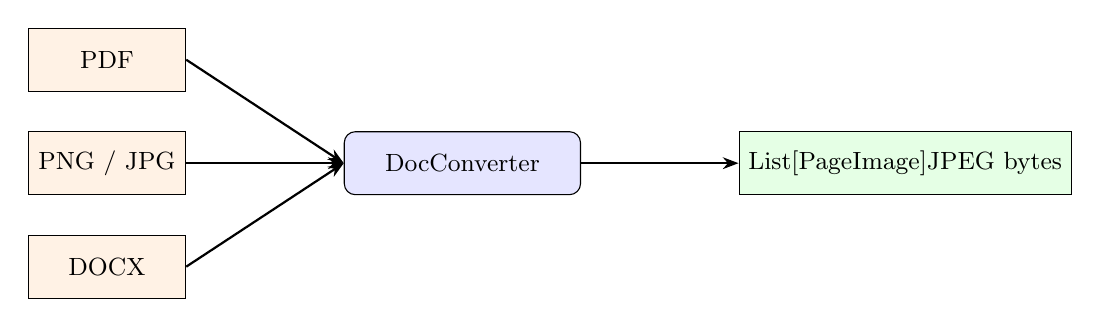
\begin{tikzpicture}[
  node distance=1.5cm and 1cm,
  input/.style={rectangle, draw, fill=orange!10, minimum width=2cm, minimum height=0.8cm, font=\small},
  process/.style={rectangle, draw, rounded corners, fill=blue!10, minimum width=3cm, minimum height=0.8cm, font=\small},
  output/.style={rectangle, draw, fill=green!10, minimum width=2.5cm, minimum height=0.8cm, font=\small},
  arrow/.style={-{Stealth[length=2mm]}, thick}
]
  \node[input] (pdf) {PDF};
  \node[input, below=0.5cm of pdf] (img) {PNG / JPG};
  \node[input, below=0.5cm of img] (docx) {DOCX};
  \node[process, right=2cm of img] (conv) {DocConverter};
  \node[output, right=2cm of conv] (out) {List[PageImage]\\JPEG bytes};

  \draw[arrow] (pdf.east) -- (conv.west);
  \draw[arrow] (img.east) -- (conv.west);
  \draw[arrow] (docx.east) -- (conv.west);
  \draw[arrow] (conv) -- (out);
\end{tikzpicture}
\end{center}

\section{PageImage 数据结构}

每个页面转换后的结果封装为 \texttt{PageImage} 数据类:

\begin{lstlisting}[caption={PageImage 定义}]
@dataclass
class PageImage:
    page_num: int       # 页码(0-based)
    png_bytes: bytes    # 实际为 JPEG 字节(历史命名)
    width_px: int       # 图片宽度(像素)
    height_px: int      # 图片高度(像素)
\end{lstlisting}

\section{PDF 转换:PyMuPDF}

PDF 是审计文档的主要格式。使用 PyMuPDF\index{PyMuPDF}(即 \texttt{fitz})库将 PDF 的每一页渲染为图片。

\subsection{渲染流程}

\begin{lstlisting}[caption={PDF 页面渲染}]
import fitz  # PyMuPDF

def _convert_pdf(self, path: str) -> list[PageImage]:
    doc = fitz.open(path)
    pages = []
    for i, page in enumerate(doc):
        # DPI 转换矩阵:72 dpi -> 目标 dpi
        mat = fitz.Matrix(self._dpi / 72, self._dpi / 72)
        pix = page.get_pixmap(matrix=mat)

        # Pixmap -> JPEG bytes
        jpeg_bytes = self._to_jpeg_bytes(pix)

        pages.append(PageImage(
            page_num=i,
            png_bytes=jpeg_bytes,
            width_px=pix.width,
            height_px=pix.height,
        ))
    doc.close()
    return pages
\end{lstlisting}

\subsection{DPI 与图片质量}

\begin{notebox}[DPI 选择的权衡]
DPI(Dots Per Inch)决定了渲染精度与文件大小的平衡:
\begin{itemize}
  \item \textbf{72 dpi}:PDF 原始分辨率,文件小但文字可能模糊
  \item \textbf{150 dpi}(推荐):清晰度足够 OCR 识别,文件大小适中
  \item \textbf{300 dpi}:高清晰度,但文件体积是 150 dpi 的 4 倍
\end{itemize}
在实际测试中,300 dpi 的大图片会导致 API 传输超时(SSL 连接中断),因此 HyperRAG 默认使用 150 dpi。
\end{notebox}

\subsection{JPEG 压缩}

为了进一步减小传输体积,将 PyMuPDF 的 Pixmap(RGB 原始像素)转换为 JPEG 格式:

\begin{lstlisting}[caption={Pixmap 转 JPEG}]
from PIL import Image
import io

def _to_jpeg_bytes(self, pix) -> bytes:
    img = Image.frombytes("RGB", (pix.width, pix.height), pix.samples)
    buf = io.BytesIO()
    img.save(buf, format="JPEG", quality=self._jpeg_quality)
    return buf.getvalue()
\end{lstlisting}

\begin{table}[htbp]
\centering
\caption{不同压缩参数对 A4 页面的影响}
\label{tab:compression}
\begin{tabular}{lcc}
\toprule
\textbf{配置} & \textbf{文件大小} & \textbf{OCR 准确率} \\
\midrule
PNG @ 300 dpi & $\sim$2-5 MB & 最高 \\
JPEG 75 @ 150 dpi & $\sim$100-300 KB & 高 \\
JPEG 50 @ 100 dpi & $\sim$30-80 KB & 中等 \\
\bottomrule
\end{tabular}
\end{table}

\section{图片处理:PIL}

对于直接上传的图片文件(PNG/JPG),处理相对简单:

\begin{lstlisting}[caption={图片文件处理}]
def _convert_image(self, path: str) -> list[PageImage]:
    img = Image.open(path).convert("RGB")
    buf = io.BytesIO()
    img.save(buf, format="JPEG", quality=self._jpeg_quality)
    return [PageImage(
        page_num=0,
        png_bytes=buf.getvalue(),
        width_px=img.width,
        height_px=img.height,
    )]
\end{lstlisting}

图片文件只有一"页",因此返回包含单个 \texttt{PageImage} 的列表。

\section{Word 文档:python-docx}

DOCX 格式\index{DOCX}是结构化的 XML 文档,不需要 OCR 即可直接提取文本。python-docx 库提供了段落级别的访问:

\begin{lstlisting}[caption={DOCX 文本提取}]
from docx import Document

def _convert_docx(self, path: str) -> list[PageImage]:
    doc = Document(path)
    full_text = "\n".join(p.text for p in doc.paragraphs if p.text.strip())
    # 将文本渲染为图片(简化处理)
    # 实际实现中,DOCX 的文本直接参与索引,
    # 图片仅用于 UI 预览
    ...
\end{lstlisting}

\begin{warnbox}[DOCX 的局限性]
python-docx 只能提取文本段落,对于 DOCX 中嵌入的图片、复杂表格,提取能力有限。如果 DOCX 包含大量视觉元素,建议先将其导出为 PDF 再处理。
\end{warnbox}

\section{统一入口:convert 方法}

\texttt{DocConverter.convert()} 方法根据文件扩展名自动选择转换策略:

\begin{lstlisting}[caption={统一转换入口}]
def convert(self, file_path: str) -> list[PageImage]:
    ext = Path(file_path).suffix.lower()
    if ext == ".pdf":
        return self._convert_pdf(file_path)
    elif ext in (".png", ".jpg", ".jpeg"):
        return self._convert_image(file_path)
    elif ext == ".docx":
        return self._convert_docx(file_path)
    else:
        raise ValueError(f"Unsupported file type: {ext}")
\end{lstlisting}

\section{实践要点}

\begin{enumerate}
  \item \textbf{内存管理}:处理大 PDF(数百页)时,应逐页渲染而非一次性加载所有页面到内存中。HyperRAG 使用 \texttt{for page in doc} 迭代器模式。
  \item \textbf{错误处理}:损坏的 PDF 或不支持的加密格式会导致 PyMuPDF 抛出异常,应在 UI 层捕获并提示用户。
  \item \textbf{临时文件}:转换后的 JPEG 字节直接存在内存中(\texttt{PageImage.png\_bytes}),不写入磁盘,避免临时文件管理问题。
  \item \textbf{尺寸记录}:\texttt{width\_px} 和 \texttt{height\_px} 在后续 BBox 坐标转换中至关重要——Vision LLM 返回的坐标是相对于这个图片尺寸的。
\end{enumerate}

\chapter{Vision LLM 与结构化 OCR}
\label{ch:vision-ocr}

\section{传统 OCR 与 Vision LLM 的区别}

传统 OCR 引擎(如 Tesseract\index{Tesseract}、PaddleOCR\index{PaddleOCR})专注于字符识别,输出的是纯文本或带坐标的文字行。而 Vision LLM 的能力远超字符识别:

\begin{table}[htbp]
\centering
\caption{传统 OCR 与 Vision LLM 的对比}
\begin{tabular}{lp{5cm}p{5cm}}
\toprule
\textbf{维度} & \textbf{传统 OCR} & \textbf{Vision LLM} \\
\midrule
输出 & 文字行 + 字符坐标 & 结构化 JSON(文本、表格、图表描述) \\
表格处理 & 需要额外的表格检测模型 & 直接输出 Markdown 表格 \\
语义理解 & 无 & 能理解上下文、推断缺失信息 \\
多语言 & 需要分别配置 & 原生多语言支持 \\
成本 & 低(本地运行) & 较高(API 调用) \\
速度 & 快 & 较慢(网络延迟 + 推理时间) \\
\bottomrule
\end{tabular}
\end{table}

\section{提示词工程:OCR 系统提示}

Vision LLM 的输出质量很大程度上取决于提示词(Prompt)的设计。HyperRAG 的 OCR 系统提示词位于 \texttt{prompts/ocr\_system.txt}:

\begin{lstlisting}[language={},caption={OCR 系统提示词},basicstyle=\small\ttfamily]
You are a high-precision document digitisation assistant.

TASK: Parse the uploaded page image. Extract ALL text
content, tables, and figures.

REQUIREMENTS:
1. For every content block, provide bounding box coordinates
   as [y_min, x_min, y_max, x_max] normalised to a 0-1000
   scale relative to the full image dimensions.
2. Tables must be converted to Markdown format.
3. Figures/charts should be described textually.
4. Preserve the reading order of the document.
5. Output ONLY valid JSON -- no markdown fences, no commentary.

OUTPUT JSON SCHEMA:
{
  "content_blocks": [
    {
      "content_type": "text" | "table" | "figure",
      "text": "<extracted text or markdown table>",
      "bbox": [y_min, x_min, y_max, x_max]
    }
  ]
}

COORDINATE RULES:
- y_min, x_min = top-left corner of the bounding box
- y_max, x_max = bottom-right corner of the bounding box
- All values are integers in the range [0, 1000]
- (0, 0) is the top-left; (1000, 1000) is the bottom-right
\end{lstlisting}

\subsection{提示词设计要点}

\begin{enumerate}
  \item \textbf{明确输出格式}——指定 JSON Schema,减少模型"自由发挥"的空间。
  \item \textbf{坐标约定}——明确 \texttt{[y\_min, x\_min, y\_max, x\_max]} 的顺序和范围。不同模型可能有不同的默认坐标约定,必须在提示词中显式说明。
  \item \textbf{内容类型枚举}——限定 \texttt{text}、\texttt{table}、\texttt{figure} 三种类型,后续处理代码只需匹配这三种。
  \item \textbf{禁止额外输出}——"Output ONLY valid JSON"防止模型在 JSON 前后添加解释性文字。
\end{enumerate}

\section{Vision API 调用}

\subsection{图片编码}

将 JPEG 字节编码为 base64 字符串,嵌入 OpenAI Vision API 的消息格式:

\begin{lstlisting}[caption={Base64 图片编码与 API 调用}]
import base64

def _parse_page(self, page: PageImage) -> PageInfo:
    b64 = base64.b64encode(page.png_bytes).decode("utf-8")

    messages = [
        {"role": "system", "content": self._system_prompt},
        {"role": "user", "content": [
            {
                "type": "text",
                "text": "Extract all content with bounding boxes "
                        "from this document page.",
            },
            {
                "type": "image_url",
                "image_url": {
                    "url": f"data:image/jpeg;base64,{b64}",
                },
            },
        ]},
    ]

    resp = self._client.chat.completions.create(
        model=self._model,
        messages=messages,
        max_tokens=self._max_tokens,
        temperature=0.0,
    )
    raw = resp.choices[0].message.content
    return self._parse_response(raw, page)
\end{lstlisting}

\begin{notebox}[temperature = 0.0 的重要性]
对于 OCR 任务,我们希望输出尽可能确定性和一致性,因此将 \texttt{temperature} 设为 0.0。这意味着模型几乎总是选择概率最高的 token,减少随机性。
\end{notebox}

\subsection{MIME 类型}

\texttt{data:image/jpeg;base64,\{b64\}} 中的 MIME 类型必须与实际图片格式匹配。由于我们在 DocConverter 中将所有图片转换为 JPEG,这里统一使用 \texttt{image/jpeg}。

\section{响应解析}

Vision LLM 的响应并不总是完美的 JSON。实践中可能遇到以下情况:

\begin{enumerate}
  \item 模型在 JSON 外面包裹了 Markdown 代码围栏(\texttt{```json ... ```})
  \item JSON 前后有解释性文字
  \item BBox 坐标超出 0-1000 范围
  \item JSON 格式错误(罕见但可能发生)
\end{enumerate}

\subsection{JSON 提取}

\texttt{\_extract\_json} 方法处理前两种情况:

\begin{lstlisting}[caption={从 LLM 响应中提取 JSON}]
import re

@staticmethod
def _extract_json(text: str) -> str:
    """Strip markdown fences and surrounding text."""
    # 尝试匹配 ```json ... ``` 代码块
    m = re.search(r"```(?:json)?\s*\n?(.*?)```", text, re.DOTALL)
    if m:
        return m.group(1).strip()

    # 回退:找到第一个 { 和最后一个 }
    start = text.find("{")
    end = text.rfind("}")
    if start != -1 and end != -1 and end > start:
        return text[start : end + 1]

    return text.strip()
\end{lstlisting}

\subsection{坐标钳位(Clamping)}

Vision LLM 有时会返回超出 0-1000 范围的坐标(如 1040),这会导致 Pydantic 验证失败。解决方案是钳位函数:

\begin{lstlisting}[caption={坐标钳位}]
def _clamp(v: int) -> int:
    return max(0, min(1000, v))

bbox = BBox(
    y_min=_clamp(int(bbox_list[0])),
    x_min=_clamp(int(bbox_list[1])),
    y_max=_clamp(int(bbox_list[2])),
    x_max=_clamp(int(bbox_list[3])),
)
\end{lstlisting}

\begin{warnbox}[防御性编程]
与 LLM 交互时,永远不要假设输出格式是完美的。即使提示词要求 "only valid JSON",模型仍可能输出非预期格式。系统的每一层都应有容错机制。
\end{warnbox}

\subsection{内容类型映射}

LLM 返回的 \texttt{content\_type} 可能有意料之外的值(如 "paragraph"、"heading"),需要映射到已定义的枚举:

\begin{lstlisting}[caption={容错的内容类型映射}]
ct_raw = item.get("content_type", "text").lower()
try:
    ct = ContentType(ct_raw)
except ValueError:
    ct = ContentType.TEXT  # 未知类型回退为 text
\end{lstlisting}

\section{逐页解析与进度反馈}

\texttt{parse\_single\_page} 方法将解析逻辑封装为单页粒度,便于 UI 层展示实时进度:

\begin{lstlisting}[caption={逐页解析}]
def parse_single_page(self, page: PageImage,
                      page_idx: int, total: int) -> PageInfo:
    t0 = time.time()
    img_kb = len(page.png_bytes) / 1024
    log.info(
        f"[OCR] Page {page_idx + 1}/{total} | "
        f"size={page.width_px}x{page.height_px} | "
        f"image={img_kb:.0f}KB | sending to {self._model}..."
    )
    page_info = self._parse_page(page)
    elapsed = time.time() - t0
    log.info(
        f"[OCR] Page {page_idx + 1}/{total} done "
        f"in {elapsed:.1f}s | "
        f"{len(page_info.content_blocks)} content blocks"
    )
    return page_info
\end{lstlisting}

在 Streamlit 层使用 \texttt{st.progress} 结合此方法:

\begin{lstlisting}[caption={UI 进度条}]
progress = st.progress(0, text="OCR parsing...")
for i, page in enumerate(pages):
    progress.progress(i / total, text=f"Page {i+1}/{total}")
    page_info = parser.parse_single_page(page, i, total)
    parsed_pages.append(page_info)
progress.progress(1.0, text="OCR complete")
\end{lstlisting}

\section{性能优化策略}

\begin{enumerate}
  \item \textbf{降低 DPI}:从 300 降到 150,图片体积减少 75\%,API 传输更快。
  \item \textbf{JPEG 压缩}:quality=75 在清晰度和体积之间取得良好平衡。
  \item \textbf{超时与重试}:设置 \texttt{httpx.Timeout(300.0, connect=30.0)} 和 \texttt{max\_retries=3},应对网络波动。
  \item \textbf{模型选择}:不同 Vision 模型的速度差异巨大。可通过修改 \texttt{config.yaml} 灵活切换。
\end{enumerate}

\chapter{向量数据库与语义检索}
\label{ch:vector-database}

\section{为什么需要向量数据库}

传统的关键词搜索(如 SQL \texttt{LIKE} 或全文索引)只能匹配字面相同的词语。而在审计场景中,用户的提问方式千变万化:

\begin{itemize}
  \item 用户问"付款金额",文档中写的是"交易总额"
  \item 用户问"签约方",文档中写的是"甲方"
  \item 用户问"违规行为",文档中描述的是具体操作细节
\end{itemize}

向量数据库\index{向量数据库}通过\textbf{语义相似度}而非字面匹配来检索,解决了这个问题。

\section{Embedding 原理}

\subsection{什么是 Embedding}

Embedding(嵌入)\index{Embedding}是将文本映射到高维向量空间的过程。在这个空间中,语义相近的文本对应的向量也相近:

\begin{center}
\begin{tikzpicture}[scale=1.5]
  \draw[->] (0,0) -- (3,0) node[right] {维度 1};
  \draw[->] (0,0) -- (0,2.5) node[above] {维度 2};

  \fill[red] (1.0, 2.0) circle (2pt) node[right, font=\small] {合同金额};
  \fill[red] (1.2, 1.8) circle (2pt) node[right, font=\small] {交易总额};
  \fill[blue] (2.5, 0.5) circle (2pt) node[right, font=\small] {签约日期};
  \fill[blue] (2.3, 0.7) circle (2pt) node[left, font=\small] {合同日期};

  \draw[<->, dashed, red!60] (1.0, 2.0) -- (1.2, 1.8);
  \draw[<->, dashed, blue!60] (2.5, 0.5) -- (2.3, 0.7);
\end{tikzpicture}
\end{center}

实际的 Embedding 向量通常有 768 或 1536 个维度,上图仅为 2D 示意。

\subsection{余弦相似度}

两个向量的相似度通常用\textbf{余弦相似度}(Cosine Similarity)\index{余弦相似度}计算:

\[
  \text{sim}(\mathbf{a}, \mathbf{b}) = \frac{\mathbf{a} \cdot \mathbf{b}}{|\mathbf{a}| \cdot |\mathbf{b}|}
\]

值域为 $[-1, 1]$,1 表示完全相同,0 表示不相关,$-1$ 表示完全相反。ChromaDB 默认使用余弦相似度进行检索。

\section{ChromaDB 基础}

ChromaDB\index{ChromaDB} 是一个嵌入式向量数据库,特点包括:

\begin{itemize}
  \item \textbf{零配置}——不需要单独部署服务器,直接嵌入 Python 进程
  \item \textbf{持久化}——使用 \texttt{PersistentClient},数据存储在本地磁盘
  \item \textbf{内置 Embedding}——默认使用 \texttt{all-MiniLM-L6-v2} 模型
  \item \textbf{元数据过滤}——支持在向量搜索的同时按元数据字段过滤
\end{itemize}

\subsection{初始化}

\begin{lstlisting}[caption={ChromaDB 初始化}]
import chromadb
from chromadb.config import Settings as ChromaSettings

class VectorStore:
    def __init__(self, persist_dir: str, collection_name: str):
        self._client = chromadb.PersistentClient(
            path=persist_dir,
            settings=ChromaSettings(
                anonymized_telemetry=False,  # 关闭遥测
            ),
        )
        self._collection = self._client.get_or_create_collection(
            name=collection_name,
            metadata={"hnsw:space": "cosine"},
        )
\end{lstlisting}

\begin{tipbox}[关闭遥测]
ChromaDB 默认发送匿名使用数据。在某些环境中,遥测的 HTTP 请求可能因依赖版本不兼容(如 posthog 库)而抛出异常。建议在生产环境中始终设置 \texttt{anonymized\_telemetry=False}。
\end{tipbox}

\section{文档索引}

将 \texttt{ParsedDocument} 的所有内容块索引到 ChromaDB:

\begin{lstlisting}[caption={文档索引实现}]
def add_document(self, doc: ParsedDocument) -> int:
    ids, documents, metadatas = [], [], []

    for page in doc.pages:
        for j, block in enumerate(page.content_blocks):
            chunk_id = f"{doc.doc_id}_p{page.page_num}_b{j}"

            ids.append(chunk_id)
            documents.append(block.text)
            metadatas.append({
                "doc_id": doc.doc_id,
                "filename": doc.filename,
                "page_num": page.page_num,
                "content_type": block.content_type.value,
                "bbox_json": block.bbox.model_dump_json(),
            })

    if ids:
        self._collection.add(
            ids=ids,
            documents=documents,
            metadatas=metadatas,
        )
    return len(ids)
\end{lstlisting}

\subsection{关键设计决策}

\begin{description}
  \item[Chunk ID 设计] 格式为 \texttt{doc\_id\_pN\_bM},确保全局唯一且可追溯到具体文档、页面、块。
  \item[BBox 元数据] 将 BBox 序列化为 JSON 字符串存入 \texttt{bbox\_json} 字段。ChromaDB 的元数据只支持基本类型(str/int/float),不支持嵌套对象。
  \item[不做额外分块] 每个 ContentBlock 就是一个 chunk。因为 Vision LLM 已经按语义单元(段落、表格、图表)做了分块,不需要再做文本切分。
\end{description}

\section{语义检索}

\begin{lstlisting}[caption={语义检索实现}]
def search(self, query: str, top_k: int = 5) -> list[RetrievalResult]:
    results = self._collection.query(
        query_texts=[query],
        n_results=top_k,
    )

    retrieval_results = []
    for i in range(len(results["ids"][0])):
        meta = results["metadatas"][0][i]
        bbox = None
        if "bbox_json" in meta:
            bbox = BBox.model_validate_json(meta["bbox_json"])

        retrieval_results.append(RetrievalResult(
            text=results["documents"][0][i],
            doc_id=meta["doc_id"],
            page_num=meta["page_num"],
            content_type=meta.get("content_type", "text"),
            bbox=bbox,
            score=1 - results["distances"][0][i],
        ))
    return retrieval_results
\end{lstlisting}

\begin{notebox}[距离与相似度的转换]
ChromaDB 返回的是\textbf{距离}(distance),而我们通常需要的是\textbf{相似度}(similarity)。对于余弦距离:
\[
  \text{similarity} = 1 - \text{distance}
\]
距离为 0 表示完全相同(相似度 = 1),距离为 2 表示完全相反(相似度 = -1)。
\end{notebox}

\section{BBox 的全链路传播}

HyperRAG 的一个核心设计理念是 \textbf{BBox 坐标贯穿整个管道}:

\begin{enumerate}
  \item \textbf{OCR 阶段}:Vision LLM 为每个内容块生成 BBox $\rightarrow$ 存入 \texttt{ContentBlock.bbox}
  \item \textbf{索引阶段}:BBox 序列化为 JSON $\rightarrow$ 存入 ChromaDB 元数据
  \item \textbf{检索阶段}:从元数据反序列化 BBox $\rightarrow$ 返回 \texttt{RetrievalResult.bbox}
  \item \textbf{Agent 阶段}:Agent 工具返回带 BBox 的检索结果 $\rightarrow$ 写入 \texttt{AuditFinding}
  \item \textbf{高亮阶段}:BBox 转换为 PDF 物理坐标 $\rightarrow$ 标注在原始 PDF 上
\end{enumerate}

这条链路确保了最终的审计发现可以精确追溯到原始文档的具体位置。

\section{实践要点}

\begin{enumerate}
  \item \textbf{幂等性}:\texttt{add\_document} 使用确定性 ID,重复添加同一文档不会产生重复记录(ChromaDB 的 upsert 语义)。
  \item \textbf{Collection 管理}:每个项目使用独立的 collection name,避免不同项目的数据互相污染。
  \item \textbf{Embedding 模型}:ChromaDB 默认使用 \texttt{all-MiniLM-L6-v2},首次运行会自动下载。如需更高质量的 Embedding,可配置其他模型。
  \item \textbf{检索数量}:\texttt{top\_k} 默认为 5,在审计场景中建议设为 5-10。过多会引入噪声,过少可能遗漏关键信息。
\end{enumerate}

\chapter{知识图谱构建}
\label{ch:knowledge-graph}

\section{为什么向量检索还不够}

向量检索擅长找到语义相关的文档片段,但有一个根本局限:\textbf{它不理解实体之间的关系}。

考虑以下审计场景:

\begin{quote}
"公司 A 的合同由张三签署,合同金额 500 万,但发票开给了公司 B,发票金额 520 万。"
\end{quote}

向量检索能找到包含"公司 A"或"500 万"的文档片段,但无法回答"张三签署的合同对应的发票是否金额一致"这类需要\textbf{关系推理}的问题。

知识图谱\index{知识图谱}(Knowledge Graph, KG)弥补了这一缺陷。它显式存储实体及其关系,支持路径查询和关系推理。

\section{实体与关系的定义}

\subsection{实体类型}

HyperRAG 定义了 7 种审计相关的实体类型:

\begin{table}[htbp]
\centering
\caption{实体类型定义}
\begin{tabular}{llp{6cm}}
\toprule
\textbf{类型} & \textbf{英文} & \textbf{示例} \\
\midrule
人物 & Person & 张三、李四、王总 \\
公司 & Company & 华为技术有限公司、腾讯 \\
金额 & Amount & 500万元、\$1,200,000 \\
日期 & Date & 2024年3月15日、Q2 2024 \\
法规 & Regulation & 《公司法》第42条、ISO 9001 \\
文档 & Document & 采购合同编号 HW-2024-001 \\
地点 & Location & 深圳市南山区、北京 \\
\bottomrule
\end{tabular}
\end{table}

\subsection{关系类型}

8 种关系类型覆盖了常见的审计关联:

\begin{table}[htbp]
\centering
\caption{关系类型定义}
\begin{tabular}{llp{5cm}}
\toprule
\textbf{关系} & \textbf{含义} & \textbf{示例} \\
\midrule
signed\_by & 签署 & 合同 $\rightarrow$ 张三 \\
issued\_by & 开具 & 发票 $\rightarrow$ 公司A \\
paid\_to & 付款 & 500万 $\rightarrow$ 公司B \\
dated & 日期关联 & 合同 $\rightarrow$ 2024-03-15 \\
regulated\_by & 受法规约束 & 采购流程 $\rightarrow$ 《采购法》 \\
located\_at & 位于 & 公司A $\rightarrow$ 深圳 \\
references & 引用 & 发票 $\rightarrow$ 合同编号 \\
amounts\_to & 金额对应 & 合同 $\rightarrow$ 500万 \\
\bottomrule
\end{tabular}
\end{table}

\subsection{数据模型}

\begin{lstlisting}[caption={Entity 和 Relation 模型}]
class Entity(BaseModel):
    name: str               # 实体名称(原文)
    entity_type: str        # 实体类型
    source_doc_id: str      # 来源文档 ID
    source_page: int        # 来源页码
    source_bbox: Optional[BBox] = None  # 来源坐标

class Relation(BaseModel):
    source_entity: str      # 源实体名称
    target_entity: str      # 目标实体名称
    relation_type: str      # 关系类型
    source_doc_id: str      # 来源文档 ID
    source_page: int        # 来源页码
\end{lstlisting}

\section{使用 LLM 提取实体与关系}

\subsection{提取提示词}

实体关系提取使用 Claude 模型,提示词位于 \texttt{prompts/entity\_extraction.txt}:

\begin{lstlisting}[language={},caption={实体提取提示词(节选)},basicstyle=\small\ttfamily]
You are an information extraction specialist.

ENTITY TYPES to extract:
- Person: names of individuals
- Company: company or organisation names
- Amount: monetary values with currency
- Date: dates, time periods, deadlines
...

RELATION TYPES to extract:
- signed_by: a document/contract signed by a person
- issued_by: a document issued by a company
...

RULES:
1. Only extract entities and relations that are
   explicitly stated in the text.
2. Each entity must include its exact name as it
   appears in the text.
...

OUTPUT JSON SCHEMA:
{
  "entities": [{"name": "...", "entity_type": "..."}],
  "relations": [{"source": "...", "target": "...",
                  "relation_type": "..."}]
}
\end{lstlisting}

\begin{warnbox}[提取准确性]
提示词中的第一条规则"Only extract entities and relations that are \textbf{explicitly stated}"至关重要。没有这条约束,LLM 可能会"推断"出文档中不存在的实体和关系,导致知识图谱中出现错误信息。
\end{warnbox}

\subsection{逐页提取}

为了控制 LLM 的输入长度和提高提取精度,采用逐页提取策略:

\begin{lstlisting}[caption={逐页实体提取}]
def extract(self, doc: ParsedDocument) -> tuple:
    all_entities, all_relations = [], []

    for page in doc.pages:
        page_text = "\n".join(
            b.text for b in page.content_blocks
        )
        if not page_text.strip():
            continue

        entities, relations = self._extract_from_page(
            doc_id=doc.doc_id,
            page_num=page.page_num,
            page_text=page_text,
            page=page,
        )
        all_entities.extend(entities)
        all_relations.extend(relations)

    # 实体去重
    all_entities = self._deduplicate_entities(all_entities)
    return all_entities, all_relations
\end{lstlisting}

\subsection{实体去重}

同一个实体可能在多个页面中出现。去重逻辑基于 (name.lower(), entity\_type.lower()) 的唯一组合:

\begin{lstlisting}[caption={实体去重}]
def _deduplicate_entities(self, entities):
    seen = {}
    for ent in entities:
        key = (ent.name.lower(), ent.entity_type.lower())
        if key not in seen:
            seen[key] = ent
    return list(seen.values())
\end{lstlisting}

\section{NetworkX 图存储}

HyperRAG 使用 NetworkX\index{NetworkX} 作为知识图谱的存储引擎。

\subsection{为什么选择 NetworkX}

\begin{table}[htbp]
\centering
\caption{图数据库选型对比}
\begin{tabular}{lp{4cm}p{4cm}}
\toprule
\textbf{方案} & \textbf{优势} & \textbf{劣势} \\
\midrule
Neo4j & 专业图数据库,Cypher 查询语言强大 & 需要单独部署,配置复杂 \\
NetworkX & 纯 Python,零部署,API 简洁 & 全在内存,不适合大规模 \\
Amazon Neptune & 托管服务,高可用 & 成本高,过重 \\
\bottomrule
\end{tabular}
\end{table}

对于 Streamlit 单用户场景,NetworkX 完全足够。

\subsection{图操作实现}

\begin{lstlisting}[caption={KnowledgeGraphStore 核心方法}]
import networkx as nx

class KnowledgeGraphStore:
    def __init__(self):
        self._graph = nx.DiGraph()  # 有向图

    def add_entities(self, entities: list[Entity]):
        for ent in entities:
            self._graph.add_node(
                ent.name,
                entity_type=ent.entity_type,
                source_doc_id=ent.source_doc_id,
                source_page=ent.source_page,
            )

    def add_relations(self, relations: list[Relation]):
        for rel in relations:
            self._graph.add_edge(
                rel.source_entity,
                rel.target_entity,
                relation_type=rel.relation_type,
                source_doc_id=rel.source_doc_id,
                source_page=rel.source_page,
            )
\end{lstlisting}

\subsection{邻居查询}

查询某个实体的 $n$ 跳邻居,用于 Agent 的关系探索:

\begin{lstlisting}[caption={邻居查询}]
def query_neighbors(self, entity: str, depth: int = 2):
    if entity not in self._graph:
        return {"nodes": [], "edges": []}

    # BFS 获取 n 跳子图
    nodes = set()
    frontier = {entity}
    for _ in range(depth):
        next_frontier = set()
        for n in frontier:
            for neighbor in (
                list(self._graph.successors(n))
                + list(self._graph.predecessors(n))
            ):
                if neighbor not in nodes:
                    next_frontier.add(neighbor)
        nodes |= frontier
        frontier = next_frontier
    nodes |= frontier

    # 构建子图
    subgraph = self._graph.subgraph(nodes)
    ...
\end{lstlisting}

\section{图谱的审计价值}

知识图谱在审计中的典型应用:

\begin{enumerate}
  \item \textbf{交叉验证}:同一笔交易在合同和发票中的金额是否一致?通过图路径连接合同实体和发票实体,比较 \texttt{amounts\_to} 关系的目标。
  \item \textbf{关系发现}:某个人同时签署了采购合同和验收报告——这是否构成利益冲突?
  \item \textbf{完整性检查}:每份合同是否都有对应的发票和验收单?检查 Document 类型节点的出边是否完整。
  \item \textbf{异常检测}:某个公司的所有合同都由同一人签署,且金额均略低于审批阈值——这是否为刻意规避审批?
\end{enumerate}

\begin{tipbox}[知识图谱 + 向量检索 = 混合搜索]
HyperRAG 的 Agent 同时拥有向量检索工具和知识图谱查询工具。这种\textbf{混合搜索}(Hybrid Search)策略让 Agent 既能找到语义相关的文本,又能追踪实体间的结构化关系,大幅提升审计推理的完整性。
\end{tipbox}

\chapter{LangGraph 审计 Agent}
\label{ch:agent}

\section{什么是 Agent}

在 LLM 应用中,Agent\index{Agent} 是一个能够\textbf{自主决定使用哪些工具、以何种顺序执行}的智能体。与简单的"用户提问 $\rightarrow$ 检索 $\rightarrow$ 生成回答"流程不同,Agent 可以:

\begin{enumerate}
  \item 分析用户问题,决定需要哪些信息
  \item 调用工具获取信息
  \item 分析工具返回的结果
  \item 决定是否需要更多信息(再次调用工具)
  \item 最终综合所有信息生成回答
\end{enumerate}

这种多步推理能力对审计场景至关重要——审计员不会只看一个文档片段就下结论,而是会交叉查证多个信息来源。

\section{ReAct 模式}

ReAct\index{ReAct}(Reasoning + Acting)是目前最流行的 Agent 架构模式。它让 LLM 在每一步交替进行\textbf{思考}(Reasoning)和\textbf{行动}(Acting):

\begin{center}
\begin{tikzpicture}[
  node distance=1cm,
  think/.style={rectangle, draw, rounded corners, fill=yellow!15,
    minimum width=4cm, minimum height=0.8cm, font=\small},
  act/.style={rectangle, draw, rounded corners, fill=blue!10,
    minimum width=4cm, minimum height=0.8cm, font=\small},
  obs/.style={rectangle, draw, rounded corners, fill=green!10,
    minimum width=4cm, minimum height=0.8cm, font=\small},
  arrow/.style={-{Stealth[length=2mm]}, thick}
]
  \node[think] (t1) {Thought: 需要查找合同金额};
  \node[act, below=of t1] (a1) {Action: search\_documents("合同金额")};
  \node[obs, below=of a1] (o1) {Observation: 找到 3 个相关片段...};
  \node[think, below=of o1] (t2) {Thought: 需要对比发票金额};
  \node[act, below=of t2] (a2) {Action: query\_knowledge\_graph("发票")};
  \node[obs, below=of a2] (o2) {Observation: 发票关联实体...};
  \node[think, below=of o2] (t3) {Thought: 发现金额不一致,生成报告};

  \draw[arrow] (t1) -- (a1);
  \draw[arrow] (a1) -- (o1);
  \draw[arrow] (o1) -- (t2);
  \draw[arrow] (t2) -- (a2);
  \draw[arrow] (a2) -- (o2);
  \draw[arrow] (o2) -- (t3);
\end{tikzpicture}
\end{center}

\section{LangGraph 框架}

LangGraph\index{LangGraph} 是 LangChain 团队开发的 Agent 框架,基于图(Graph)的概念组织 Agent 的执行流程。

\subsection{为什么选择 LangGraph}

\begin{itemize}
  \item \textbf{原生 ReAct 支持}——\texttt{create\_react\_agent} 一行代码即可创建完整的 ReAct Agent
  \item \textbf{流式输出}——原生支持流式返回中间步骤,适合 UI 实时显示推理过程
  \item \textbf{状态管理}——自动管理对话历史和工具调用状态
  \item \textbf{可扩展}——可以轻松添加自定义节点和边
\end{itemize}

\subsection{Agent 创建}

\begin{lstlisting}[caption={创建 ReAct Agent}]
from langgraph.prebuilt import create_react_agent

class AuditAgent:
    def __init__(self, llm, tools, prompts_dir, max_iterations):
        self._system_prompt = self._load_prompt(prompts_dir)
        self._max_iterations = max_iterations

        self._agent = create_react_agent(
            model=llm,
            tools=tools,
            prompt=self._system_prompt,
        )
\end{lstlisting}

\section{工具设计}

Agent 的能力由其可用工具决定。HyperRAG 为审计 Agent 设计了 5 个专用工具:

\subsection{工具清单}

\begin{table}[htbp]
\centering
\caption{Agent 工具清单}
\begin{tabular}{lp{8cm}}
\toprule
\textbf{工具名称} & \textbf{功能} \\
\midrule
\texttt{search\_documents} & 在向量数据库中进行语义搜索,返回最相关的文档片段及其 BBox \\
\texttt{query\_knowledge\_graph} & 查询知识图谱中某个实体的邻居节点和关系 \\
\texttt{query\_graph\_path} & 查询两个实体之间的连接路径 \\
\texttt{get\_page\_content} & 获取指定文档的指定页面的完整内容 \\
\texttt{list\_entities\_by\_type} & 列出知识图谱中某类型的所有实体 \\
\bottomrule
\end{tabular}
\end{table}

\subsection{工具实现示例}

使用 LangChain 的 \texttt{@tool} 装饰器定义工具:

\begin{lstlisting}[caption={search\_documents 工具}]
from langchain_core.tools import tool

def create_tools(vector_store, kg_store, parsed_docs):

    @tool
    def search_documents(query: str) -> str:
        """Search documents by semantic similarity.
        Returns relevant text chunks with source info."""
        results = vector_store.search(query, top_k=5)
        if not results:
            return "No relevant documents found."
        output = []
        for r in results:
            output.append(
                f"[Doc:{r.doc_id} Page:{r.page_num+1} "
                f"Score:{r.score:.2f}]\n{r.text[:500]}"
            )
        return "\n---\n".join(output)

    @tool
    def query_knowledge_graph(entity_name: str) -> str:
        """Query the knowledge graph for an entity's
        relationships and neighbors."""
        result = kg_store.query_neighbors(
            entity_name, depth=2
        )
        if not result["nodes"]:
            return f"Entity '{entity_name}' not found."
        return json.dumps(result, ensure_ascii=False,
                          indent=2)

    ...
    return [search_documents, query_knowledge_graph,
            query_graph_path, get_page_content,
            list_entities_by_type]
\end{lstlisting}

\begin{notebox}[工具 Docstring 的重要性]
LLM 通过工具的 \textbf{docstring}(函数文档字符串)来理解工具的用途和使用方式。一个好的 docstring 应该:
\begin{itemize}
  \item 清晰描述工具的功能
  \item 说明输入参数的含义
  \item 描述返回值的格式
\end{itemize}
LLM 会根据 docstring 决定何时使用哪个工具以及传入什么参数。
\end{notebox}

\subsection{工厂模式}

工具通过 \texttt{create\_tools} 工厂函数创建,接收依赖项作为参数。这种模式的优势:

\begin{enumerate}
  \item \textbf{依赖注入}——工具函数通过闭包访问 \texttt{vector\_store}、\texttt{kg\_store} 等对象,不依赖全局变量。
  \item \textbf{可测试性}——单元测试可以传入 mock 对象。
  \item \textbf{解耦}——工具定义与存储实现分离。
\end{enumerate}

\section{流式推理}

审计查询的推理过程可能持续数十秒,为了让用户了解 Agent 的工作进展,使用流式输出:

\begin{lstlisting}[caption={流式推理输出}]
def stream(self, query: str):
    """Yield reasoning steps as they happen."""
    inputs = {"messages": [("user", query)]}
    config = {"recursion_limit": self._max_iterations * 2}

    for event in self._agent.stream(inputs, config):
        for node_name, node_output in event.items():
            messages = node_output.get("messages", [])
            for msg in messages:
                if hasattr(msg, "tool_calls") and msg.tool_calls:
                    for tc in msg.tool_calls:
                        yield {
                            "type": "tool_call",
                            "content": f"{tc['name']}({tc['args']})"
                        }
                elif hasattr(msg, "content") and msg.content:
                    if msg.type == "tool":
                        yield {
                            "type": "tool_result",
                            "content": msg.content[:500]
                        }
                    else:
                        yield {
                            "type": "thinking",
                            "content": msg.content
                        }
\end{lstlisting}

在 Streamlit 中,每个 yield 的步骤会实时显示在界面上,用户可以看到 Agent 正在调用哪个工具、获取了什么结果。

\section{审计报告生成}

Agent 的最终输出是一个结构化的审计报告:

\begin{lstlisting}[language=json,caption={审计报告 JSON 结构}]
{
  "findings": [
    {
      "finding_id": "F001",
      "description": "合同金额与发票总额不一致",
      "severity": "high",
      "evidence": [
        "合同 HW-2024-001 金额为 500 万元",
        "对应发票总额为 520 万元"
      ],
      "source_pages": [
        {"doc_id": "abc123", "page_num": 3}
      ],
      "related_entities": ["HW-2024-001", "500万元"]
    }
  ],
  "summary": "发现 1 项高风险问题..."
}
\end{lstlisting}

\subsection{报告解析}

与 OCR 响应类似,Agent 输出的 JSON 也需要容错解析:

\begin{lstlisting}[caption={报告解析}]
def _parse_report(self, query: str, content: str):
    cleaned = self._extract_json(content)
    try:
        data = json.loads(cleaned)
    except json.JSONDecodeError:
        return AuditReport(
            query=query,
            findings=[],
            summary=content,  # 回退:将原文作为摘要
        )
    # 构建 AuditReport...
\end{lstlisting}

\section{Agent 系统提示词}

位于 \texttt{prompts/audit\_system.txt} 的系统提示词定义了 Agent 的角色和行为准则:

\begin{enumerate}
  \item \textbf{角色定义}——"You are an expert financial and compliance auditor AI assistant"
  \item \textbf{工具说明}——列出所有可用工具及其用途
  \item \textbf{工作流程}——理解 $\rightarrow$ 搜索 $\rightarrow$ 交叉验证 $\rightarrow$ 识别异常 $\rightarrow$ 生成报告
  \item \textbf{输出格式}——JSON Schema 定义
  \item \textbf{行为规则}——引用具体页码、分级严重程度、不捏造证据
\end{enumerate}

\begin{tipbox}[迭代次数限制]
\texttt{max\_iterations} 限制了 Agent 的最大推理步数(默认 10 步)。这是一个安全阀——防止 Agent 陷入无限循环。在实践中,大多数审计查询在 3-6 步内完成。
\end{tipbox}

\chapter{PDF 溯源高亮}
\label{ch:highlighting}

\section{溯源的意义}

在审计工作中,"证据在哪里"与"发现了什么"同样重要。传统 RAG 系统只能返回文本片段,审计员还需要手动在原始文档中定位证据。HyperRAG 通过 PDF 高亮标注实现了\textbf{自动溯源}——点击"在 PDF 中查看",即可看到证据在原始文档上被高亮标出。

这个功能的实现依赖于一条关键的数据链路:

\begin{center}
\begin{tikzpicture}[
  node distance=0.5cm and 1cm,
  box/.style={rectangle, draw, rounded corners, fill=blue!8,
    minimum width=3.5cm, minimum height=0.8cm, font=\small, align=center},
  arrow/.style={-{Stealth[length=2mm]}, thick}
]
  \node[box] (v) {Vision LLM\\BBox [0-1000]};
  \node[box, right=1.5cm of v] (s) {ChromaDB\\元数据存储};
  \node[box, right=1.5cm of s] (a) {Agent\\AuditFinding};
  \node[box, below=1cm of a] (c) {坐标转换\\BBox $\rightarrow$ PDFRect};
  \node[box, left=1.5cm of c] (h) {PyMuPDF\\PDF 标注};

  \draw[arrow] (v) -- (s);
  \draw[arrow] (s) -- (a);
  \draw[arrow] (a) -- (c);
  \draw[arrow] (c) -- (h);
\end{tikzpicture}
\end{center}

\section{坐标系统}

系统中涉及三个不同的坐标系统:

\subsection{Vision LLM 归一化坐标}

Vision LLM 返回的 BBox 是归一化到 0-1000 的整数坐标:

\begin{itemize}
  \item 原点 $(0, 0)$:页面\textbf{左上角}
  \item 终点 $(1000, 1000)$:页面\textbf{右下角}
  \item 格式:$[\text{y\_min}, \text{x\_min}, \text{y\_max}, \text{x\_max}]$
\end{itemize}

\subsection{PDF 坐标系统}

PDF 使用\textbf{点}(Point, 1 pt = 1/72 inch)作为单位,但坐标原点在\textbf{左下角}:

\begin{itemize}
  \item 原点 $(0, 0)$:页面\textbf{左下角}
  \item $x$ 轴向右,$y$ 轴\textbf{向上}
  \item A4 纸张尺寸:$595.28 \times 841.89$ pt
\end{itemize}

\subsection{PyMuPDF 坐标系统}

PyMuPDF(fitz)使用的坐标系与 PDF 原始坐标\textbf{不同}:

\begin{itemize}
  \item 原点 $(0, 0)$:页面\textbf{左上角}
  \item $y$ 轴\textbf{向下}(与 PDF 原始坐标相反)
  \item 单位仍为点(pt)
\end{itemize}

\begin{notebox}[坐标系对比]
\begin{center}
\begin{tikzpicture}[scale=0.8]
  % Vision LLM
  \draw (0,0) rectangle (2.5,3.5);
  \fill[red] (0,3.5) circle (2pt);
  \node[above right, font=\small] at (0,3.5) {(0,0)};
  \node[below left, font=\small] at (2.5,0) {(1000,1000)};
  \draw[->] (0,3.5) -- (0,2.5) node[left,font=\tiny]{y};
  \draw[->] (0,3.5) -- (1,3.5) node[above,font=\tiny]{x};
  \node[below, font=\small\bfseries] at (1.25,-0.3) {Vision LLM};

  % PyMuPDF
  \begin{scope}[xshift=4cm]
  \draw (0,0) rectangle (2.5,3.5);
  \fill[blue] (0,3.5) circle (2pt);
  \node[above right, font=\small] at (0,3.5) {(0,0)};
  \node[below left, font=\small] at (2.5,0) {(W,H)};
  \draw[->] (0,3.5) -- (0,2.5) node[left,font=\tiny]{y};
  \draw[->] (0,3.5) -- (1,3.5) node[above,font=\tiny]{x};
  \node[below, font=\small\bfseries] at (1.25,-0.3) {PyMuPDF (pt)};
  \end{scope}

  % PDF native
  \begin{scope}[xshift=8cm]
  \draw (0,0) rectangle (2.5,3.5);
  \fill[green!50!black] (0,0) circle (2pt);
  \node[below right, font=\small] at (0,0) {(0,0)};
  \node[above left, font=\small] at (2.5,3.5) {(W,H)};
  \draw[->] (0,0) -- (0,1) node[left,font=\tiny]{y};
  \draw[->] (0,0) -- (1,0) node[below,font=\tiny]{x};
  \node[below, font=\small\bfseries] at (1.25,-0.3) {PDF 原生 (pt)};
  \end{scope}
\end{tikzpicture}
\end{center}
Vision LLM 和 PyMuPDF 的坐标原点相同(左上角),$y$ 轴方向也相同(向下),因此转换相对简单。
\end{notebox}

\section{坐标转换算法}

由于 Vision LLM 和 PyMuPDF 的坐标原点和 $y$ 轴方向一致,转换公式较为直接:

\begin{align}
  x_0^{\text{pdf}} &= \frac{x_\text{min}}{1000} \times W_{\text{page}} \label{eq:x0} \\
  y_0^{\text{pdf}} &= \frac{y_\text{min}}{1000} \times H_{\text{page}} \label{eq:y0} \\
  x_1^{\text{pdf}} &= \frac{x_\text{max}}{1000} \times W_{\text{page}} \label{eq:x1} \\
  y_1^{\text{pdf}} &= \frac{y_\text{max}}{1000} \times H_{\text{page}} \label{eq:y1}
\end{align}

其中 $W_{\text{page}}$ 和 $H_{\text{page}}$ 是 PDF 页面的宽度和高度(单位:点)。

\begin{lstlisting}[caption={坐标转换实现}]
import fitz

def gemini_bbox_to_pdf_rect(
    bbox: BBox,
    page: fitz.Page,
) -> fitz.Rect:
    """Convert normalised [0-1000] bbox to PDF Rect."""
    pw = page.rect.width
    ph = page.rect.height

    x0 = (bbox.x_min / 1000) * pw
    y0 = (bbox.y_min / 1000) * ph
    x1 = (bbox.x_max / 1000) * pw
    y1 = (bbox.y_max / 1000) * ph

    return fitz.Rect(x0, y0, x1, y1)
\end{lstlisting}

\section{PDF 高亮标注}

使用 PyMuPDF 的注释(Annotation)API 在 PDF 上添加高亮:

\begin{lstlisting}[caption={PDF 高亮实现}]
class PDFHighlighter:
    def highlight(
        self,
        pdf_path: str,
        locations: list[PDFRect],
        output_path: str,
        color: tuple = (1, 1, 0),    # 黄色
        opacity: float = 0.35,
    ) -> str:
        doc = fitz.open(pdf_path)

        for loc in locations:
            if loc.page_num >= len(doc):
                continue

            page = doc[loc.page_num]
            rect = fitz.Rect(loc.x0, loc.y0, loc.x1, loc.y1)

            # 添加高亮注释
            annot = page.add_highlight_annot(rect)
            annot.set_colors(stroke=color)
            annot.set_opacity(opacity)
            annot.update()

        doc.save(output_path)
        doc.close()
        return output_path
\end{lstlisting}

\subsection{高亮参数}

\begin{description}
  \item[color] RGB 三元组,范围 $[0, 1]$。默认 $(1, 1, 0)$ 为黄色。审计中也可使用红色 $(1, 0, 0)$ 标注高风险发现。
  \item[opacity] 透明度,范围 $[0, 1]$。0.35 是一个折中值——既能清晰看到高亮,又不遮挡原文。
\end{description}

\section{从 AuditFinding 到高亮 PDF}

完整的高亮流程:

\begin{enumerate}
  \item Agent 返回 \texttt{AuditFinding},其中 \texttt{source\_locations} 包含一组 \texttt{PDFRect}(已转换的 PDF 物理坐标)。
  \item UI 层调用 \texttt{PDFHighlighter.highlight()},传入原始 PDF 路径和坐标列表。
  \item PyMuPDF 在每个坐标位置添加高亮注释。
  \item 高亮后的 PDF 保存到 \texttt{data/highlighted/} 目录。
  \item UI 将高亮 PDF 以 base64 内嵌到 \texttt{<iframe>} 中显示。
\end{enumerate}

\begin{lstlisting}[caption={UI 层的高亮调用}]
def _show_highlighted_pdf(finding):
    for loc in finding.source_locations:
        for doc_id, path in st.session_state.file_paths.items():
            if path.lower().endswith(".pdf"):
                output = os.path.join(
                    settings.highlighted_dir,
                    f"highlighted_{finding.finding_id}.pdf",
                )
                highlighter.highlight(
                    pdf_path=path,
                    locations=finding.source_locations,
                    output_path=output,
                )
                # 显示高亮 PDF
                pdf_bytes = Path(output).read_bytes()
                b64 = base64.b64encode(pdf_bytes).decode()
                st.markdown(
                    f'<iframe src="data:application/pdf;'
                    f'base64,{b64}" width="100%" '
                    f'height="500"></iframe>',
                    unsafe_allow_html=True,
                )
\end{lstlisting}

\section{精度与误差}

BBox 坐标的精度受多个因素影响:

\begin{enumerate}
  \item \textbf{Vision LLM 的坐标精度}——不同模型的坐标精度不同,通常在 $\pm20$(相当于页面尺寸的 2\%)。
  \item \textbf{DPI 转换}——页面图片的 DPI 不影响归一化坐标,但影响 LLM 的"视觉分辨率"。
  \item \textbf{钳位截断}——超出 0-1000 范围的坐标被钳位到边界,可能导致高亮区域偏小。
\end{enumerate}

\begin{tipbox}[实践建议]
在实际使用中,建议对 BBox 做适当的\textbf{扩展}(如四边各扩展 10-20 个归一化单位),确保高亮区域完整覆盖目标内容,即使坐标有轻微偏差也不会遗漏。
\end{tipbox}

\chapter{Streamlit Web 界面}
\label{ch:web-ui}

\section{为什么选择 Streamlit}

构建 RAG 系统的 Web 界面有多种选择:

\begin{table}[htbp]
\centering
\caption{Web 框架对比}
\begin{tabular}{lp{4cm}p{4cm}}
\toprule
\textbf{框架} & \textbf{优势} & \textbf{劣势} \\
\midrule
Streamlit & 纯 Python,快速原型,内置组件丰富 & 定制性有限,不适合复杂交互 \\
Gradio & 专为 ML Demo 设计,简单易用 & 布局灵活性差 \\
Flask + React & 完全自定义,前后端分离 & 开发成本高 \\
FastAPI + Vue & 高性能 API,现代前端 & 技术栈复杂 \\
\bottomrule
\end{tabular}
\end{table}

对于 HyperRAG 这类数据分析导向的应用,Streamlit\index{Streamlit} 是最佳选择:

\begin{itemize}
  \item 100\% Python,无需前端开发经验
  \item 内置文件上传、进度条、表格、PDF 嵌入等组件
  \item \texttt{st.session\_state} 自动管理应用状态
  \item 修改代码后自动刷新,开发效率极高
\end{itemize}

\section{应用结构}

HyperRAG 的 Streamlit 应用采用\textbf{侧边栏 + 三 Tab} 的布局:

\begin{lstlisting}[caption={应用主框架}]
def main() -> None:
    st.set_page_config(
        page_title="HyperRAG Audit",
        layout="wide",
    )
    _init_session_state()

    with st.sidebar:
        render_sidebar()

    tab_docs, tab_audit, tab_graph = st.tabs(
        [t("tab_docs"), t("tab_audit"), t("tab_graph")]
    )

    with tab_docs:
        render_document_view()
    with tab_audit:
        render_audit_query()
    with tab_graph:
        render_knowledge_graph()
\end{lstlisting}

\begin{description}
  \item[侧边栏] 语言切换、文件上传、已上传文档列表、重建知识图谱按钮
  \item[Tab 1: 文档预览] 原始 PDF 与解析内容的双栏对比
  \item[Tab 2: 审计查询] 查询输入、Agent 推理过程、审计发现与 PDF 高亮
  \item[Tab 3: 知识图谱] 交互式图谱可视化、实体搜索与过滤
\end{description}

\section{Session State 管理}

Streamlit 的每次用户交互都会重新执行整个脚本。为了在交互之间保持状态,使用 \texttt{st.session\_state}:

\begin{lstlisting}[caption={Session State 初始化}]
def _init_session_state() -> None:
    if "initialised" in st.session_state:
        return  # 已初始化,跳过

    settings = Settings()

    # 创建所有服务实例
    factory = LLMClientFactory(
        api_key=settings.zenmux_api_key,
        base_url=settings.zenmux_base_url,
    )
    st.session_state.settings = settings
    st.session_state.factory = factory
    st.session_state.openai_client = factory.get_openai_client()
    st.session_state.claude_llm = factory.get_langchain_llm(
        model=settings.claude_model,
    )
    st.session_state.doc_converter = DocConverter(...)
    st.session_state.gemini_parser = GeminiParser(...)
    st.session_state.vector_store = VectorStore(...)
    st.session_state.kg_store = KnowledgeGraphStore()
    ...

    st.session_state.parsed_docs = {}   # doc_id -> ParsedDocument
    st.session_state.uploaded_files = {}  # filename -> doc_id
    st.session_state.file_paths = {}      # doc_id -> file path
    st.session_state.kg_built = False

    st.session_state.initialised = True
\end{lstlisting}

\begin{notebox}[初始化守卫模式]
\texttt{if "initialised" in st.session\_state: return} 这个模式确保了昂贵的初始化操作(如创建数据库连接、加载配置)只执行一次。每次用户点击按钮或切换 Tab 时,脚本重新执行但会跳过初始化。
\end{notebox}

\section{文件上传与处理流程}

上传流程是应用中最复杂的部分,涉及多个异步步骤和进度反馈:

\begin{lstlisting}[caption={上传处理流程}]
if uploaded and st.button(t("upload_btn"), type="primary"):
    for f in uploaded:
        # Step 1: 保存文件
        save_path = os.path.join(settings.upload_dir, f.name)
        with open(save_path, "wb") as fp:
            fp.write(f.getbuffer())

        # Step 2: 转换为页面图片
        with st.status(t("converting", name=f.name)):
            pages = doc_converter.convert(save_path)

        # Step 3: 逐页 OCR(带进度条)
        progress = st.progress(0, text="OCR...")
        parsed_pages = []
        for i, page in enumerate(pages):
            progress.progress(i / total,
                text=t("ocr_progress", cur=i+1, total=total))
            page_info = parser.parse_single_page(page, i, total)
            parsed_pages.append(page_info)
        progress.progress(1.0, text=t("ocr_done"))

        # Step 4: 向量索引
        n = vector_store.add_document(parsed)

        # Step 5: 知识图谱构建(带进度条)
        kg_progress = st.progress(0, text="KG...")
        for i, page in enumerate(parsed.pages):
            kg_progress.progress(i / total, ...)
            ents, rels = extractor._extract_from_page(...)
            ...
        kg_progress.progress(1.0)
\end{lstlisting}

\subsection{进度反馈设计}

HyperRAG 使用两种进度反馈机制:

\begin{enumerate}
  \item \textbf{st.status}——用于简短的同步操作(如文件转换),显示为可展开的状态卡片。
  \item \textbf{st.progress}——用于逐页处理的长操作(如 OCR 和 KG 构建),显示为进度条并实时更新文本。
\end{enumerate}

\section{国际化(i18n)}

HyperRAG 支持中英文切换,采用字典映射方案:

\begin{lstlisting}[caption={i18n 实现}]
I18N = {
    "en": {
        "page_title": "HyperRAG Audit",
        "upload_header": "Upload Documents",
        "upload_btn": "Upload & Parse",
        ...
    },
    "zh": {
        "page_title": "HyperRAG 智能审计",
        "upload_header": "上传文档",
        "upload_btn": "上传并解析",
        ...
    },
}

def t(key: str, **kwargs) -> str:
    """Get translated string for current language."""
    lang = st.session_state.get("lang", "zh")
    text = I18N.get(lang, I18N["en"]).get(key, key)
    if kwargs:
        text = text.format(**kwargs)
    return text
\end{lstlisting}

\texttt{t()} 函数支持参数插值:\texttt{t("ocr\_progress", cur=3, total=10)} 会渲染为 "OCR: 正在解析第 3/10 页..."。

\section{知识图谱可视化}

使用 \texttt{streamlit-agraph}\index{streamlit-agraph} 库实现交互式图谱:

\begin{lstlisting}[caption={知识图谱可视化}]
from streamlit_agraph import agraph, Node, Edge, Config

# 为每个实体类型定义颜色
type_colors = {
    "Person": "#2e7d32",
    "Company": "#1565c0",
    "Amount": "#e65100",
    ...
}

# 使用数值 ID 避免 CJK 字符的 URL 编码问题
name_to_id = {n["name"]: f"n{i}" for i, n in enumerate(nodes_data)}

nodes = [
    Node(
        id=name_to_id[n["name"]],
        label=n["name"][:20],  # 截断长标签
        size=25,
        color=type_colors.get(n.get("entity_type"), "#999"),
        title=f'{n.get("entity_type")}: {n["name"]}',
    )
    for n in nodes_data
]

edges = [
    Edge(
        source=name_to_id[e["source"]],
        target=name_to_id[e["target"]],
        label=e.get("relation_type", ""),
    )
    for e in edges_data
]

config = Config(
    width=900, height=500,
    directed=True, physics=True,
)
agraph(nodes=nodes, edges=edges, config=config)
\end{lstlisting}

\begin{warnbox}[CJK 字符的坑]
\texttt{streamlit-agraph} 内部将节点 ID 用于 URL 路径。如果 ID 包含中文字符,会导致 \texttt{FileNotFoundError}。解决方案是使用数值 ID(如 \texttt{n0}, \texttt{n1}),将中文名称放在 \texttt{label} 和 \texttt{title} 属性中。
\end{warnbox}

\section{PDF 内嵌显示}

Streamlit 没有原生的 PDF 查看器组件,使用 HTML \texttt{<iframe>} 内嵌 base64 编码的 PDF:

\begin{lstlisting}[caption={PDF 内嵌显示}]
pdf_bytes = Path(file_path).read_bytes()
b64 = base64.b64encode(pdf_bytes).decode()
pdf_html = (
    f'<iframe src="data:application/pdf;base64,{b64}" '
    f'width="100%" height="600" '
    f'type="application/pdf"></iframe>'
)
st.markdown(pdf_html, unsafe_allow_html=True)
\end{lstlisting}

\begin{tipbox}[unsafe\_allow\_html]
\texttt{unsafe\_allow\_html=True} 允许注入原始 HTML。仅在你完全控制 HTML 内容时使用。不要将用户输入直接拼入 HTML 字符串,防止 XSS 攻击。
\end{tipbox}

\chapter{配置管理与部署}
\label{ch:deployment}

\section{配置管理}

\subsection{为什么需要外部配置}

将 API Key、模型名称、路径等参数硬编码在代码中会带来诸多问题:

\begin{enumerate}
  \item \textbf{安全风险}——API Key 可能泄露到版本控制系统
  \item \textbf{环境差异}——开发环境和生产环境需要不同的配置
  \item \textbf{灵活性差}——切换模型或调整参数需要修改代码
\end{enumerate}

HyperRAG 使用 \texttt{config.yaml} 作为外部配置文件,通过 \texttt{.gitignore} 排除,确保敏感信息不进入代码仓库。

\subsection{YAML 配置结构}

\begin{lstlisting}[language=yaml,caption={config.yaml 完整结构}]
# ZenMux API 设置
# 注册获取 API Key: https://zenmux.ai/invite/GBQMC5
api:
  base_url: "https://zenmux.ai/api/v1"
  api_key: "sk-your-api-key-here"

# 模型配置
models:
  ocr_model: "openai/gpt-5.2-chat"
  agent_model: "anthropic/claude-sonnet-4"

# 解析器设置
parser:
  dpi: 150
  jpeg_quality: 75
  max_tokens: 4096

# 向量数据库设置
vectordb:
  persist_dir: "data/chroma_db"
  collection_name: "hyperrag_docs"

# Agent 设置
agent:
  max_iterations: 10

# 数据目录
paths:
  upload_dir: "data/uploads"
  parsed_dir: "data/parsed"
  highlighted_dir: "data/highlighted"
  prompts_dir: "prompts"
\end{lstlisting}

\subsection{配置加载器}

\texttt{Settings} 类从 YAML 文件加载所有配置,并将相对路径解析为绝对路径:

\begin{lstlisting}[caption={Settings 配置加载器}]
import yaml
from pathlib import Path

_PROJECT_ROOT = Path(__file__).resolve().parent.parent
_CONFIG_PATH = _PROJECT_ROOT / "config.yaml"

class Settings:
    def __init__(self, config_path=None):
        path = Path(config_path) if config_path else _CONFIG_PATH
        if not path.exists():
            raise FileNotFoundError(
                f"Config file not found: {path}"
            )

        with open(path, encoding="utf-8") as f:
            cfg = yaml.safe_load(f)

        # API
        api = cfg.get("api", {})
        self.zenmux_base_url = api.get(
            "base_url", "https://zenmux.ai/api/v1"
        )
        self.zenmux_api_key = api.get("api_key", "")

        # Models
        models = cfg.get("models", {})
        self.gemini_model = models.get(
            "ocr_model", "openai/gpt-5.2-chat"
        )
        self.claude_model = models.get(
            "agent_model", "anthropic/claude-sonnet-4"
        )

        # Paths -- resolve relative to project root
        paths = cfg.get("paths", {})
        self.upload_dir = str(
            _PROJECT_ROOT / paths.get("upload_dir", "data/uploads")
        )
        ...
\end{lstlisting}

\begin{tipbox}[yaml.safe\_load 与 yaml.load]
始终使用 \texttt{yaml.safe\_load()} 而非 \texttt{yaml.load()}。后者允许执行任意 Python 代码(通过 YAML 的 \texttt{!!python/object} 标签),存在代码注入风险。
\end{tipbox}

\subsection{配置模板}

仓库中包含 \texttt{config.yaml.example} 作为模板,用户复制后填入自己的 API Key:

\begin{lstlisting}[language={},basicstyle=\small\ttfamily,frame=none,numbers=none]
$ cp config.yaml.example config.yaml
$ vim config.yaml  # 填入 API Key
\end{lstlisting}

\section{LLM 客户端工厂}

\texttt{LLMClientFactory} 封装了 LLM 客户端的创建逻辑,处理超时、重试等网络配置:

\begin{lstlisting}[caption={LLM 客户端工厂}]
import httpx
from openai import OpenAI
from langchain_openai import ChatOpenAI

class LLMClientFactory:
    def __init__(self, api_key: str, base_url: str):
        self._api_key = api_key
        self._base_url = base_url

    def get_openai_client(self) -> OpenAI:
        """Raw OpenAI client for Vision API."""
        return OpenAI(
            api_key=self._api_key,
            base_url=self._base_url,
            timeout=httpx.Timeout(300.0, connect=30.0),
            max_retries=3,
        )

    def get_langchain_llm(self, model: str) -> ChatOpenAI:
        """LangChain wrapper for Agent."""
        return ChatOpenAI(
            model=model,
            api_key=self._api_key,
            base_url=self._base_url,
            temperature=0.0,
        )
\end{lstlisting}

\subsection{超时与重试策略}

\begin{description}
  \item[连接超时 30s] 如果 30 秒内无法建立 TCP 连接,认为网络不可达。
  \item[总超时 300s] Vision OCR 对大页面的处理可能需要较长时间,5 分钟是合理上限。
  \item[最大重试 3 次] 网络波动导致的临时失败会自动重试。
\end{description}

\section{ZenMux API 网关}

HyperRAG 的所有 LLM 调用都通过 ZenMux\index{ZenMux} 统一 API 网关完成。

\subsection{注册与获取 API Key}

\begin{enumerate}
  \item 访问 \url{https://zenmux.ai/invite/GBQMC5}
  \item 注册账户
  \item 在控制台获取 API Key(格式:\texttt{sk-...})
  \item 将 API Key 填入 \texttt{config.yaml}
\end{enumerate}

\subsection{模型命名规范}

ZenMux 的模型名称格式为 \texttt{provider/model-name}:

\begin{table}[htbp]
\centering
\caption{ZenMux 可用模型示例}
\begin{tabular}{lll}
\toprule
\textbf{模型名称} & \textbf{供应商} & \textbf{用途} \\
\midrule
\texttt{openai/gpt-5.2-chat} & OpenAI & Vision OCR \\
\texttt{anthropic/claude-sonnet-4} & Anthropic & Agent 推理 \\
\texttt{google/gemini-3-pro-preview} & Google & Vision OCR(备选) \\
\texttt{anthropic/claude-opus-4} & Anthropic & 复杂推理 \\
\bottomrule
\end{tabular}
\end{table}

切换模型只需修改 \texttt{config.yaml},无需改动任何代码。

\section{目录结构与 .gitignore}

\subsection{运行时数据目录}

\begin{lstlisting}[language={},basicstyle=\small\ttfamily,frame=none,numbers=none,
  caption={data/ 目录结构}]
data/
|-- uploads/       # 用户上传的原始文件
|-- parsed/        # OCR 解析结果 (JSON)
|-- highlighted/   # 高亮标注后的 PDF
`-- chroma_db/     # ChromaDB 持久化数据
\end{lstlisting}

所有 \texttt{data/} 子目录都被 \texttt{.gitignore} 排除。

\subsection{.gitignore 策略}

\begin{lstlisting}[language={},caption={.gitignore},basicstyle=\small\ttfamily,frame=none,numbers=none]
.env                # 环境变量(备用)
config.yaml         # 包含 API Key 的配置文件
__pycache__/        # Python 字节码缓存
*.pyc
data/uploads/       # 用户数据
data/parsed/
data/highlighted/
data/chroma_db/     # 向量数据库
.venv/              # 虚拟环境
*.egg-info/
dist/
build/
\end{lstlisting}

\section{生产环境部署建议}

\subsection{Docker 部署}

\begin{lstlisting}[language={},caption={Dockerfile 示例},basicstyle=\small\ttfamily]
FROM python:3.11-slim

WORKDIR /app
COPY requirements.txt .
RUN pip install --no-cache-dir -r requirements.txt

COPY . .

EXPOSE 8501

CMD ["streamlit", "run", "app.py", \
     "--server.port=8501", \
     "--server.address=0.0.0.0"]
\end{lstlisting}

\subsection{环境变量覆盖}

在容器化部署中,可以通过环境变量覆盖 \texttt{config.yaml} 中的敏感配置,只需修改 \texttt{Settings} 类添加环境变量优先级:

\begin{lstlisting}[caption={环境变量优先级}]
import os

self.zenmux_api_key = os.getenv(
    "ZENMUX_API_KEY",
    api.get("api_key", ""),
)
\end{lstlisting}

\subsection{性能考虑}

\begin{enumerate}
  \item \textbf{并发}——Streamlit 原生是单线程的。对于多用户场景,考虑部署多个实例并使用负载均衡。
  \item \textbf{ChromaDB}——嵌入式模式只支持单进程访问。多实例部署时需使用 ChromaDB Server 模式或切换到 Qdrant 等客户端-服务器架构的向量数据库。
  \item \textbf{NetworkX}——内存中的图数据在进程重启后丢失。生产环境应考虑将图序列化到磁盘或使用 Neo4j。
  \item \textbf{文件存储}——\texttt{data/} 目录应挂载为持久化卷(Docker Volume),避免容器重启后数据丢失。
\end{enumerate}

\section{扩展方向}

HyperRAG 作为一个教学项目,展示了 RAG 审计系统的核心架构。在生产化过程中,可以考虑以下扩展:

\begin{enumerate}
  \item \textbf{异步 OCR}——使用 Celery 或 asyncio 并行处理多个页面的 OCR,大幅缩短处理时间。
  \item \textbf{增量更新}——当文档更新时,只重新解析和索引变化的页面,而非整份文档。
  \item \textbf{用户认证}——集成 OAuth 或 LDAP,支持多用户隔离。
  \item \textbf{审计模板}——预定义常见审计场景的查询模板,降低使用门槛。
  \item \textbf{导出功能}——将审计报告导出为 PDF 或 Excel,便于分发。
  \item \textbf{多模型对比}——同时调用多个 LLM 进行 OCR,取共识结果以提高准确率。
\end{enumerate}

\begin{notebox}[总结]
本书从零开始,系统地介绍了构建企业级 RAG 审计系统所需的全部知识:文档处理、Vision OCR、向量检索、知识图谱、Agent 推理、PDF 溯源高亮、Web 界面以及配置部署。每个章节都结合 HyperRAG 的实际代码进行讲解,读者可以对照源码加深理解。

完整源码:\url{https://github.com/bennix/HyperRAGAudit}

LLM API:\url{https://zenmux.ai/invite/GBQMC5}
\end{notebox}


\backmatter
\printindex

\end{document}
